\documentclass{article}

\usepackage[most]{tcolorbox}
\usepackage{physics}
\usepackage{graphicx}
\usepackage{float}
\usepackage{amsmath}
\usepackage{amssymb}


\usepackage[utf8]{inputenc}
\usepackage[a4paper, margin=1in]{geometry} % Controla los márgenes
\usepackage{titling}

\title{Tarea \#1 Relatividad General Physics Latam }
\author{Manuel Angel Garcia M.}
\date{\today}

\renewcommand{\maketitlehooka}{%
  \centering
  \vspace*{0.05cm} % Espacio vertical antes del título
}

\renewcommand{\maketitlehookd}{%
  \vspace*{2cm} % Espacio vertical después de la fecha
}

\newcommand{\caja}[3]{%
  \begin{tcolorbox}[colback=#1!5!white,colframe=#1!25!black,title=#2]
    #3
  \end{tcolorbox}%
}

\begin{document}
\maketitle

\section{Manifold Diferencial}

\textbf{a)} 
\begin{itemize}
  \item \textbf{Espacio Topológico } Sea $ X  $ un conjunto y sea $ T  $ una colección de subconjuntos de $ X  $. Se llama espacio topológico a $ (X,T) $ si cumplen las siguientes propiedades:
    \begin{itemize}
      \item $ \emptyset $ y $ X  $ están en $ T  $.
      \item Para $ \{u_i \in T \ | \ i\in I \}, \quad \underset{i }{\bigcup}\  u_i \in T $
      \item Si $ u_1,u_2 \in T \ \rightarrow \ u_1 \cap u_2 \in T $
    \end{itemize}
    $ T  $ es llamado topología.
  \item \textbf{Manifold Diferenciables } Sea $ M $ un espacio de Haussdorff, $ M  $ es un manifold diferenciables si tiene la siguiente estructura:
    \begin{itemize}
      \item Sea $ M = U_\alpha U_\alpha $ de un recubrimiento abierto
      \item Hay un mapa continuo e invertible $ \phi_\alpha \ : \ u_\alpha \ \rightarrow \ \phi_\alpha(u_\alpha) \subseteq \mathbb{R}^n $
      \item Para todo $ \alpha,\beta $ tenemos $ \phi_\alpha(u_\alpha\cap u_\beta) $ es abierto en $ \mathbb{R}^n  $, y las funciones de transición: 
        \begin{gather*}
          \phi_\alpha \circ \phi_\beta ^ {-1 }: \ \phi_\beta(u_\alpha \cap u_\beta) \ \rightarrow \ \phi_\alpha(u_\alpha \cap u_\beta)
        \end{gather*}
        Son $ C^\infty $-funciones. $ (u_\alpha, \phi_\alpha) $ es llamado un chart de coordenadas y $ \{(u_\alpha, \phi_\alpha)\}_\alpha $ es llamado Atlas.
    \end{itemize}
  \item \textbf{Manifold Diferenciable con Frontera} Es un espacio topológico que es localmente isomorfo a $ \mathbb{R}^n  $ o al \textit{half-space} $ H^n = \{\vec x \in \mathbb{R}^n \ | \ x^n \geq 0\} $ para $ 0\leq i \leq n $.
\end{itemize}

\hfill

\textbf{b)} La definición de $ S^n $
\begin{gather*}
  S^n = \{x \in \mathbb{R} ^ {n + 1 } \ |\  || x || = 1\} 
\end{gather*}
\begin{itemize}
  \item \textbf{Hausdorff } La esfera $ S^n  $ es un subespacio de $  \mathbb{R}^ {n+ 1 } $ el cual es un espacio de Hausdorff por lo que $ S^n  $ también es Hausdorff.
  \item \textbf{Base Contable } La esfera $ S^n  $ es un subespacio de $ \mathbb{R}^ {n+1 } $ el cual tiene una base contable por lo tanto $ S^n  $ también es contable.
\end{itemize}




        


\section{Difeomorfismo}

\textbf{a)} Tenemos: 
\begin{figure}[H]
    \centering
    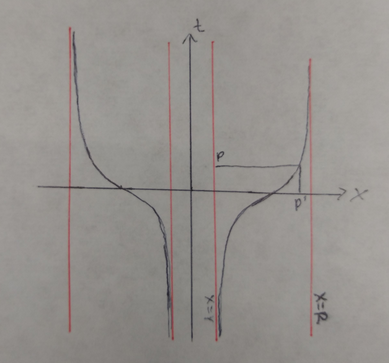
\includegraphics[width=0.40\linewidth]{cilindro.png}
\end{figure}

\begin{gather}
    t = \tan{\left[ \left(x - \frac{R+r }{2}\right)\frac{\pi }{R-r} \right]} \qquad \qquad x = \frac{R+r }{2} + \frac{R - r }{\pi }\tan ^ {-1 } t 
\end{gather}

El mapeo es: 
\begin{gather*}
    \theta' = \theta \qquad \qquad \quad  t' = \frac{R+r }{2} + \frac{R - r }{\pi }\tan ^ {-1 } t 
\end{gather*}

$ \theta' = \theta  $ claramente es suave. 

Para $ t' $:
\begin{gather*}
    \frac{d t' }{d t} = \left(\frac{R-r }{\pi } \right) \frac{1 }{1 + t^2 } \qquad 
    \frac{d ^2 t'  }{d t } =  \left(\frac{R-r }{\pi } \right) \frac{2t }{(1 + t^2)^2 } \qquad 
    \frac{d ^3 t'  }{d t ^3} = \left(\frac{R-r }{\pi } \right) \frac{6t^2 - 2 }{(1 + t^2)^3}
\end{gather*}

Cuando sigamos derivando solo se van a añadir potencias mayores en el numerador por lo que $ t'  $ es suave.

\hfill 

\textbf{b)}

\hfill 

\textbf{c)} Sea $ M,N  $ manifolds suaves con atlas $ \{U_\alpha, \phi_\alpha\} \ \ \{V_\beta, \psi_\beta\} $ con mapa $ f: M\ \rightarrow \ N  $
\begin{gather*}
    \psi_\beta \circ f \circ (\phi_\alpha)^ {-1 } : \ \phi_\alpha(U_\alpha \ \cap \ f ^ {-1 }(v)) \ \rightarrow  \ \psi_\beta(V_\beta) \qquad \text{Es suave} 
\end{gather*}
\begin{figure}[H]
    \centering
    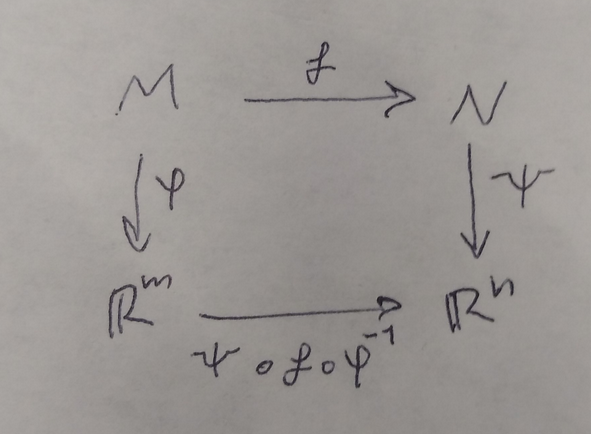
\includegraphics[width=0.40\linewidth]{suave.png}
\end{figure}
Como el mapeo $ f  $ va de un subespacio euclidiano a otro subespacio euclidiano entonces el mapeo $ f  $ debe ser suave.

\hfill 









\section{Coordenadas esferoidales }
\begin{align*}
x &= r \sinh \chi \sin \theta \cos \varphi \\
y &= r \sinh \chi \sin \theta \sin \varphi \\
z &= r \cosh \chi \cos \theta
\end{align*}

\textbf{a)} 
\[
\frac{\partial (x, y, z)}{\partial (\chi, \theta, \varphi)} = 
\begin{pmatrix}
r \cosh \chi \sin \theta \cos \varphi & r \sinh \chi \cos \theta \cos \varphi & -r \sinh \chi \sin \theta \sin \varphi \\
r \cosh \chi \sin \theta \sin \varphi & r \sinh \chi \cos \theta \sin \varphi & r \sinh \chi \sin \theta \cos \varphi \\
r \sinh \chi \cos \theta & -r \cosh \chi \sin \theta & 0
\end{pmatrix}
\]

\hfill 

\textbf{b) } Tenemos que el elemento de linea es:
\begin{gather*}
    ds^2 = (dx)^2 +(dy)^2 +(dz)^2 
\end{gather*}

De la matriz de transformación obtenemos que: 
\begin{gather*}
    dx = r \cosh \chi \sin \theta \cos \varphi \, d\chi + r \sinh \chi \cos \theta \cos \varphi \, d\theta - r \sinh \chi \sin \theta \sin \varphi \, d\varphi\\
    dy = r \cosh \chi \sin \theta \sin \varphi \, d\chi + r \sinh \chi \cos \theta \sin \varphi \, d\theta + r \sinh \chi \sin \theta \cos \varphi \, d\varphi \\
    dz = r \sinh \chi \cos \theta \, d\chi - r \cosh \chi \sin \theta \, d\theta
\end{gather*}

Reemplazando en $ ds^2 $: 
\begin{gather*}
     ds^2 =  r^2 (\sin^2 \theta +\sinh^2\chi) \, d\chi^2 + r^2(\sin^2 \theta +\sinh^2\chi) \, d\theta^2 + r^2\sinh^2 \chi \sin^2 \theta \, d\varphi^2
\end{gather*}

\hfill 

\textbf{c) }
\begin{gather*}
    g _{\chi\chi } = h^2_\chi =  r^2 (\sin^2 \theta +\sinh^2\chi) \qquad g _{\theta\theta }  = h_\theta^2 = r^2(\sin^2 \theta +\sinh^2\chi) \qquad g _{\phi\phi }  = h_\phi^2 =  r^2\sinh^2 \chi \sin^2 \theta
\end{gather*}








\section{Curvas en el ESpacio Euclidiano }
\[\begin{aligned}
    x^i(\lambda) & = (\lambda, (\lambda - 1)^2, -\lambda)\\
x^i(\mu) & = (\cos \mu, \sin \mu, \mu - 1)\\
x^i(\sigma) & = (\sigma^2, \sigma^3 + \sigma^2, \sigma)
\end{aligned}
\]
\begin{gather*}
    p : \ (x,y,z) = (1,0,-1) 
\end{gather*}

\textbf{a) } 
\begin{align*}
    \left. \frac{d x^i  }{d \lambda}\right| _{\lambda=1 } &= (1,0,-1) \\ 
        \left. \frac{d x^i  }{d \mu}\right| _{\mu=1 }&= (- \sin{\mu }, \cos{\mu }, 1 ) _{\mu = 0 }  = (0,1,1) \\ 
            \left. \frac{d x^i  }{d \sigma}\right| _{\sigma=1 }&= ( 2\sigma, 3\sigma^3 + 2 \sigma , 1  ) _{\sigma = -1}  = (-2,1,1)
\end{align*}

\hfill 

\textbf{b) } para $ f = x ^2 + y ^2 + z ^2 $

Tenemos que 
\begin{gather*}
    \frac{\partial f }{\partial x} = 2x \qquad \qquad \frac{\partial f  }{\partial y} = 2y-z \qquad \qquad \frac{\partial f  }{\partial z } = -y  
\end{gather*}

\begin{itemize}
    \item 
        \begin{gather*}
            \frac{d f }{d \lambda} = \frac{\partial f  }{\partial  x } \frac{d x  }{d \lambda} + \frac{\partial f  }{\partial  y } \frac{d y  }{d \lambda} + \frac{\partial f  }{\partial  z } \frac{d z  }{d \lambda} \\
            \frac{d x }{d \lambda} = 1 \qquad \qquad 
            \frac{d y  }{d \lambda} = 2(\lambda-1) \qquad \qquad 
            \frac{d z  }{d \lambda} = -1  \\
            \text{Reemplazando y evaluando en el punto }p\\
            \left. \frac{d f }{d \lambda} \right| _{p} = 2\lambda = 2  
        \end{gather*}
    \item 
        \begin{gather*}
            \frac{d f }{d \mu} = \frac{\partial f  }{\partial  x } \frac{d x  }{d \mu} + \frac{\partial f  }{\partial  y } \frac{d y  }{d \mu} + \frac{\partial f  }{\partial  z } \frac{d z  }{d \mu} \\
            \frac{d x }{d \mu} = -\sin{\mu} \qquad \qquad 
            \frac{d y  }{d \mu} = \cos{\mu} \qquad \qquad 
            \frac{d z  }{d \mu} = 1  \\
            \text{Reemplazando y evaluando en el punto }p\\
            \left. \frac{d f }{d \mu} \right| _{p} = -2 \cos{\mu } + \cos{\mu } = 1  
        \end{gather*}
    \item 
        \begin{gather*}
            \frac{d f }{d \sigma} = \frac{\partial f  }{\partial  x } \frac{d x  }{d \sigma} + \frac{\partial f  }{\partial  y } \frac{d y  }{d \sigma} + \frac{\partial f  }{\partial  z } \frac{d z  }{d \sigma} \\
            \frac{d x }{d \sigma} = 2\sigma \qquad \qquad 
            \frac{d y  }{d \sigma} = 3\sigma^2 + 2 \sigma \qquad \qquad 
            \frac{d z  }{d \sigma} = 1  \\
            \text{Reemplazando y evaluando en el punto }p\\
            \left. \frac{d f }{d \sigma} \right| _{p} = 6\sigma + 3 \sigma^2 = -3 
        \end{gather*}
\end{itemize}







\section{Vectores y Tensores }
\[
X^{\mu\nu} =
\begin{pmatrix}
2 & 0 & 1 & -1 \\
-1 & 0 & 3 & 2 \\
-1 & 1 & 0 & 0 \\
-2 & 1 & 1 & -2
\end{pmatrix}
 \qquad \qquad
 V^\mu = (-1, 2, 0, -2)
\]

\textbf{a) } 
\begin{gather*}
    X ^ {\mu} _{\nu} =
    \begin{pmatrix}
    -2 & 0 & 1 & -1 \\
    1 & 0 & 3 & 2 \\
    1 & 1 & 0 & 0 \\
    2 & 1 & 1 & -2
    \end{pmatrix}
\end{gather*}

\hfill 

\textbf{b) } 
\begin{gather*}
    X _ {\mu} ^{\nu} =
    \begin{pmatrix}
    -2 & 0 & -1 & 1 \\
    -1 & 0 & 3 & 2 \\
    -1 & 1 & 0 & 0 \\
    -2 & 1 & 1 & -2
    \end{pmatrix}
\end{gather*}

\hfill 

\textbf{c) } 
\begin{gather*}
    X ^ {(\mu\nu)} =
    \begin{pmatrix}
    2 & -\frac{1}{2} & 0 & -\frac{3}{2} \\
    -\frac{1}{2} & 0 & 2 & \frac{3}{2} \\
    0 & 2 & 0 & \frac{1}{2} \\
    -\frac{3}{2} & \frac{3}{2} & \frac{1}{2} & -2
    \end{pmatrix}
\end{gather*}

\hfill 

\textbf{d) } 
\begin{gather*}
    X _ {[\mu\nu]} =
    \begin{pmatrix}
    0 & -\frac{1}{2} & -1 & -\frac{1}{2} \\
    \frac{1}{2} & 0 & 1 & \frac{1}{2} \\
    1 & -1 & 0 & -\frac{1}{2} \\
    \frac{1}{2} & -\frac{1}{2} & \frac{1}{2} & 0
    \end{pmatrix}
\end{gather*}

\hfill 

\textbf{e) } 
\begin{gather*}
    X ^\lambda _ {\lambda} = -4
\end{gather*}

\hfill 

\textbf{f) } 
\begin{gather*}
    V ^ {\mu} V _{\mu}  = 7
\end{gather*}

\hfill 

\textbf{g) } 
\begin{gather*}
    V _ {\mu} X ^{\mu\nu}  = \left[4, -2, 5, 7\right]
\end{gather*}






\section{Derivada de Lie }

\textbf{a) } Formula general: $ (\mathcal{L}_x \omega)(Y) = X(\omega(y)) - \omega([X,Y]) $
\begin{align*}
  [X,Y] = X ^ {\nu} \partial_\nu Y ^ {\mu} - Y ^ {\nu} \partial_\nu X ^ {\mu} \qquad \qquad X(\omega(Y)) = X ^ {\mu} \partial _{\mu} (\omega _{\nu} Y ^ {\nu})
\end{align*}

Reemplazando en la formula general:
\begin{align*}
  (\mathcal{L}_{X } \omega) (Y) &= X(\omega(Y)) - \omega([X,Y])\\
                 &= X ^ {\mu} \partial _{\mu} (\omega _{\nu}  Y ^ {\nu}) - \omega _{\mu} (X ^ {\nu} \partial _{\nu} Y ^ {\mu} - Y ^ {\nu} \partial _{\nu}  X ^ {\mu}) \\
                 &= (X ^ {\mu} \partial _{\mu} \omega _{\nu} + \omega _{\mu}\partial _{\nu} X ^ {\mu}) Y ^ {\nu} 
\end{align*}

Por lo tanto llegamos a que:
\begin{gather*}
  (\mathcal{L}_{X } \omega) _{\nu}  = X ^ {\mu} \partial_\mu \omega_\nu + \omega_\mu \partial_\nu X ^ {\mu}
\end{gather*}

\hfill 

\hfill

\textbf{b) } para un tensor $ (0,g) \ \ g  $.

\hfill

De la formula general: $ \qquad (\mathcal{L}_x g)(Y,Z) = X(g(Y,Z)) - g([X,Y],Z) - g(X,[Y,Z]) $

\hfill 

Tomando en cuenta que $ \qquad Y = \partial_\mu \qquad Z = \partial_\nu \qquad [X,\partial_\mu] = [X^\mu\partial_\mu, \partial_\rho] = - (\partial_\rho X^\mu)\partial_\mu $

\hfill 

reemplazando lo anterior en la formula general: 
\begin{align*}
  (\mathcal{L}_X g) _{\mu\nu} &= X(g(\partial_\mu, \partial_\nu)) - g([X,\partial_\mu],\partial_\nu) - g(\partial_\mu, [X,\partial_\nu]) \\
                &= X ^ {\rho} \partial_\rho g _{\mu\nu}  + \partial_\rho X ^ {\mu} g _{\mu\nu} + \partial_\nu X ^ {\rho} g _{\mu\rho} 
\end{align*}


\end{document}
